\normaltrue
\correctiontrue

%\UPSTIidClasse{11} % 11 sup, 12 spé
%\newcommand{\UPSTIidClasse}{12}

\exer{Mouvement RR  $\star$ \label{B2:12:04}}
\setcounter{question}{0}\UPSTIcompetence{B2-12}
\index{Compétence B2-12}
\index{Mécanisme à 2 rotations}
\ifcorrection
\else
\textbf{Pas de corrigé pour cet exercice.}
\fi

\ifprof
\else
Soit le mécanisme suivant. On a $\vect{AB}=R\vect{i_1}$ avec $R=\SI{20}{mm}$ et  
$\vect{BC}=L\vect{i_2}$ avec $L=\SI{15}{mm}$.
\begin{center}
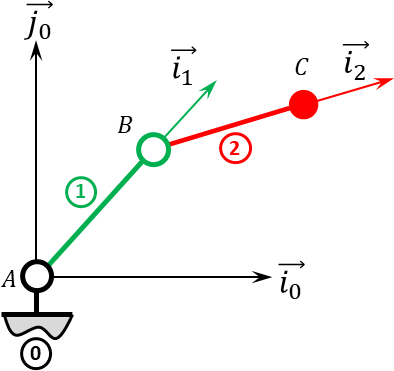
\includegraphics[width=\linewidth]{04_RR_01}
\end{center}
\fi

\question{Tracer le graphe des liaisons.}
\ifprof
\begin{center}
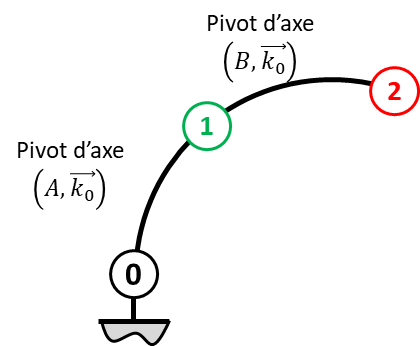
\includegraphics[width=.2\linewidth]{04_RR_01_c}
\end{center}
\else
\fi


\ifprof
\begin{multicols}{3}
\else
\fi

\question{Retracer le schéma cinématique pour $\theta=\dfrac{\pi}{4}\,\text{rad}$ et $\varphi=\pi\,\text{rad}$.}
\ifprof
\begin{center}
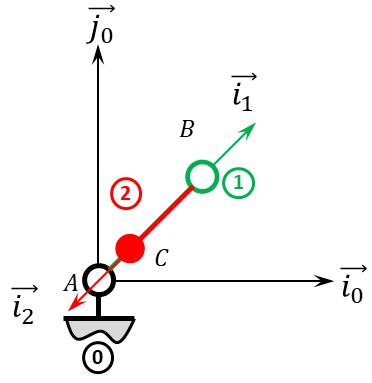
\includegraphics[width=.6\linewidth]{04_RR_02_c}
\end{center}
\else
\fi

\question{Retracer le schéma cinématique pour $\theta=\dfrac{\pi}{4}\,\text{rad}$ et $\varphi=-\dfrac{\pi}{4}\,\text{rad}$.}
\ifprof
\begin{center}
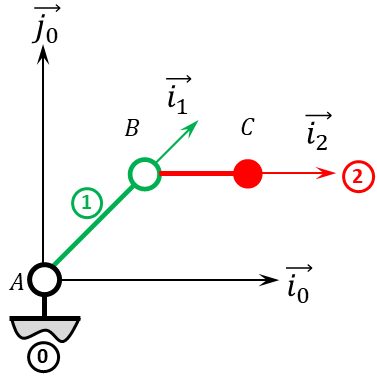
\includegraphics[width=.6\linewidth]{04_RR_03_c}
\end{center}
\else
\fi


\question{Retracer le schéma cinématique pour $\theta=\dfrac{3\pi}{4}\,\text{rad}$ et $\varphi=-\dfrac{\pi}{4}\,\text{rad}$.}
\ifprof
\begin{center}
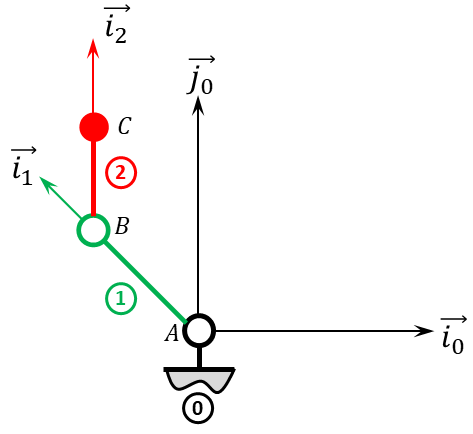
\includegraphics[width=.6\linewidth]{04_RR_04_c}
\end{center}
\else
\fi

\ifprof
\end{multicols}
\else
\fi

\ifprof
\else
\begin{flushright}
\footnotesize{Corrigé  voir \ref{B2:12:04}.}
\end{flushright}%
\fi